\documentclass[11pt,a4paper]{article}
\usepackage[utf8]{inputenc}
\usepackage[T1]{fontenc}
\usepackage{amsmath,amssymb,amsfonts}
\usepackage{graphicx}
\usepackage{tikz}
\usetikzlibrary{arrows.meta,positioning,calc,3d}
\usepackage{algorithm}
\usepackage{algpseudocode}
\usepackage{hyperref}
\usepackage{geometry}
\geometry{margin=2.5cm}

\title{Match3D v2: 2.5D Registration Algorithm\\[0.5em]\large Technical Documentation}
\author{Match3D Development Team}
\date{May 2026}

\begin{document}
\maketitle

\begin{abstract}
This document describes the registration algorithms implemented in Match3D v2 for aligning 2.5D depth images (heightmaps). Unlike standard 3D point cloud registration methods, our approach treats the problem as a 2D registration in the $(x,y)$ plane with separate handling of the $z$ (depth) axis. This design decision addresses the fundamental scale imbalance present in 2.5D data where depth values are orders of magnitude larger than lateral coordinates.
\end{abstract}

\tableofcontents
\newpage

%=============================================================================
\section{Introduction}
%=============================================================================

\subsection{The 2.5D Data Model}

A 2.5D depth image (heightmap or range image) represents a surface as a regular grid of depth measurements. Each pixel at grid position $(c, r)$ stores a single depth value $z(r, c)$. The 3D coordinates of a point are:

\begin{equation}
\mathbf{p}(r,c) = \begin{pmatrix} x \\ y \\ z \end{pmatrix} = \begin{pmatrix} c \cdot \Delta_x \\ r \cdot \Delta_y \\ z(r,c) \end{pmatrix}
\end{equation}

where $\Delta_x$ and $\Delta_y$ are the pixel sizes in meters.

\subsection{The Scale Imbalance Problem}

For typical dental surface scans:
\begin{itemize}
    \item Lateral pixel size: $\Delta_x, \Delta_y \approx 30\,\mu\text{m} = 3 \times 10^{-5}\,\text{m}$
    \item Image dimensions: $\sim 500 \times 1000$ pixels
    \item Lateral extent: $x_{\max} \approx 0.015\,\text{m}$, $y_{\max} \approx 0.03\,\text{m}$
    \item Depth values: $z \approx 800\text{--}1000\,\mu\text{m}$ (with arbitrary baseline offset)
\end{itemize}

This creates a \textbf{scale imbalance} where $z \gg x, y$. Standard 3D registration algorithms (ICP, Horn's method) compute rotations based on 3D Euclidean distances, causing the large $z$ values to dominate and produce erroneous rotations.

%=============================================================================
\section{Registration Pipeline Overview}
%=============================================================================

The registration pipeline consists of three stages:

\begin{enumerate}
    \item \textbf{Coarse Registration} -- Initial alignment using either:
    \begin{itemize}
        \item Center of Mass (COM) translation only
        \item Landmark point pairs (2D rotation + translation + $z$ offset)
    \end{itemize}

    \item \textbf{Fine Registration (Match)} -- Iterative 2.5D refinement

    \item \textbf{Difference Calculation} -- Compute per-pixel height differences
\end{enumerate}

\begin{figure}[h]
\centering
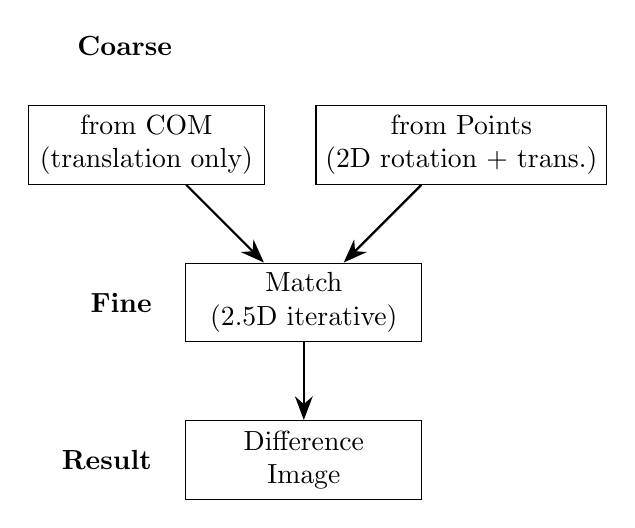
\begin{tikzpicture}[
    box/.style={rectangle, draw, minimum width=3cm, minimum height=1cm, align=center},
    arrow/.style={-{Stealth[length=3mm]}, thick}
]
    \node[box] (com) at (0,0) {from COM\\(translation only)};
    \node[box] (pts) at (4,0) {from Points\\(2D rotation + trans.)};
    \node[box] (match) at (2,-2) {Match\\(2.5D iterative)};
    \node[box] (diff) at (2,-4) {Difference\\Image};

    \draw[arrow] (com) -- (match);
    \draw[arrow] (pts) -- (match);
    \draw[arrow] (match) -- (diff);

    \node[above=0.5cm of com, anchor=south west, xshift=-1cm] {\textbf{Coarse}};
    \node[left=0.3cm of match] {\textbf{Fine}};
    \node[left=0.3cm of diff] {\textbf{Result}};
\end{tikzpicture}
\caption{Registration pipeline overview}
\end{figure}

%=============================================================================
\section{Transformation Model}
%=============================================================================

For 2.5D data, we restrict the transformation to:
\begin{itemize}
    \item Rotation around the $z$-axis only (yaw angle $\alpha$)
    \item Translation in all three axes $(t_x, t_y, t_z)$
\end{itemize}

The transformation from data coordinates to model (reference) coordinates is:

\begin{equation}
\begin{pmatrix} x' \\ y' \\ z' \end{pmatrix} =
\begin{pmatrix}
\cos\alpha & -\sin\alpha & 0 \\
\sin\alpha & \cos\alpha & 0 \\
0 & 0 & 1
\end{pmatrix}
\begin{pmatrix} x \\ y \\ z \end{pmatrix}
+
\begin{pmatrix} t_x \\ t_y \\ t_z \end{pmatrix}
\label{eq:transform}
\end{equation}

Or in compact form:
\begin{equation}
\mathbf{p}' = \mathbf{R}_z(\alpha) \cdot \mathbf{p} + \mathbf{t}
\end{equation}

%=============================================================================
\section{Coarse Registration: Center of Mass (COM)}
%=============================================================================

The simplest coarse alignment translates the data image so its center of mass coincides with the reference image's center of mass.

\subsection{Algorithm}

Given model image $M$ and data image $D$ with optional ROI masks:

\begin{equation}
\mathbf{c}_M = \frac{1}{|S_M|} \sum_{(r,c) \in S_M} \mathbf{p}_M(r,c), \quad
\mathbf{c}_D = \frac{1}{|S_D|} \sum_{(r,c) \in S_D} \mathbf{p}_D(r,c)
\end{equation}

where $S_M$ and $S_D$ are the sets of valid pixels within the ROI.

The translation is simply:
\begin{equation}
\mathbf{t} = \mathbf{c}_M - \mathbf{c}_D = \begin{pmatrix} t_x \\ t_y \\ t_z \end{pmatrix}
\end{equation}

with $\alpha = 0$ (no rotation).

%=============================================================================
\section{Coarse Registration: From Points (Landmark-Based)}
%=============================================================================

When corresponding landmark points are available, we can compute both rotation and translation.

\subsection{Problem Formulation}

Given $n$ corresponding point pairs:
\begin{itemize}
    \item Data points: $\{\mathbf{d}_i\}_{i=1}^n$ with $\mathbf{d}_i = (x_i^d, y_i^d, z_i^d)^T$
    \item Reference points: $\{\mathbf{r}_i\}_{i=1}^n$ with $\mathbf{r}_i = (x_i^r, y_i^r, z_i^r)^T$
\end{itemize}

Find $\alpha$ and $\mathbf{t}$ that minimize:
\begin{equation}
E = \sum_{i=1}^n \|\mathbf{r}_i - (\mathbf{R}_z(\alpha) \cdot \mathbf{d}_i + \mathbf{t})\|^2
\end{equation}

\subsection{2D Rotation Estimation}

\textbf{Key insight:} For 2.5D data, we solve the rotation using only the $(x,y)$ coordinates, ignoring $z$ entirely.

\subsubsection{Step 1: Compute 2D Centroids}

\begin{equation}
\bar{x}^d = \frac{1}{n}\sum_{i=1}^n x_i^d, \quad \bar{y}^d = \frac{1}{n}\sum_{i=1}^n y_i^d
\end{equation}
\begin{equation}
\bar{x}^r = \frac{1}{n}\sum_{i=1}^n x_i^r, \quad \bar{y}^r = \frac{1}{n}\sum_{i=1}^n y_i^r
\end{equation}

\subsubsection{Step 2: Center the Points}

\begin{equation}
\tilde{x}_i^d = x_i^d - \bar{x}^d, \quad \tilde{y}_i^d = y_i^d - \bar{y}^d
\end{equation}
\begin{equation}
\tilde{x}_i^r = x_i^r - \bar{x}^r, \quad \tilde{y}_i^r = y_i^r - \bar{y}^r
\end{equation}

\subsubsection{Step 3: Optimal 2D Rotation Angle}

The optimal rotation angle that minimizes the 2D alignment error is:

\begin{equation}
\boxed{\alpha = \arctan2\left(\sum_{i=1}^n (\tilde{x}_i^d \tilde{y}_i^r - \tilde{y}_i^d \tilde{x}_i^r), \sum_{i=1}^n (\tilde{x}_i^d \tilde{x}_i^r + \tilde{y}_i^d \tilde{y}_i^r)\right)}
\label{eq:2d_rotation}
\end{equation}

\textbf{Derivation:} This follows from the Procrustes problem in 2D. The optimal rotation minimizes:
\begin{equation}
E_{2D} = \sum_{i=1}^n \left[(\tilde{x}_i^r - \tilde{x}_i^d\cos\alpha + \tilde{y}_i^d\sin\alpha)^2 + (\tilde{y}_i^r - \tilde{x}_i^d\sin\alpha - \tilde{y}_i^d\cos\alpha)^2\right]
\end{equation}

Taking $\frac{\partial E_{2D}}{\partial \alpha} = 0$ yields Equation~\ref{eq:2d_rotation}.

\begin{figure}[h]
\centering
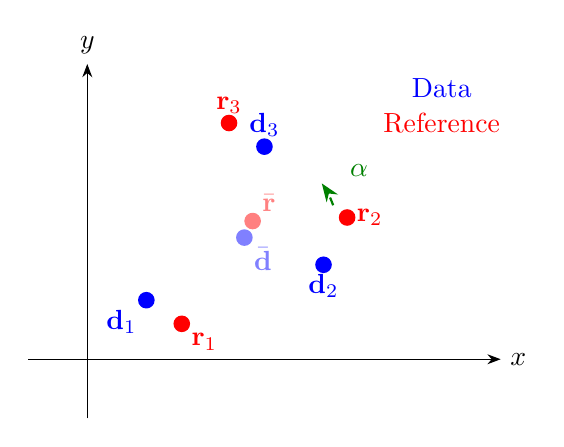
\begin{tikzpicture}[scale=1.5]
    % Coordinate system
    \draw[-{Stealth}] (-0.5,0) -- (3.5,0) node[right] {$x$};
    \draw[-{Stealth}] (0,-0.5) -- (0,2.5) node[above] {$y$};

    % Data points (before rotation)
    \fill[blue] (0.5,0.5) circle (2pt) node[below left] {$\mathbf{d}_1$};
    \fill[blue] (2,0.8) circle (2pt) node[below] {$\mathbf{d}_2$};
    \fill[blue] (1.5,1.8) circle (2pt) node[above] {$\mathbf{d}_3$};

    % Data centroid
    \fill[blue!50] (1.33,1.03) circle (2pt) node[below right] {$\bar{\mathbf{d}}$};

    % Reference points
    \fill[red] (0.8,0.3) circle (2pt) node[below right] {$\mathbf{r}_1$};
    \fill[red] (2.2,1.2) circle (2pt) node[right] {$\mathbf{r}_2$};
    \fill[red] (1.2,2) circle (2pt) node[above] {$\mathbf{r}_3$};

    % Reference centroid
    \fill[red!50] (1.4,1.17) circle (2pt) node[above right] {$\bar{\mathbf{r}}$};

    % Rotation arc
    \draw[-{Stealth},dashed,thick,green!50!black] (1.33,1.03) ++(20:0.8) arc (20:35:0.8);
    \node[green!50!black] at (2.3,1.6) {$\alpha$};

    % Legend
    \node[blue] at (3,2.3) {Data};
    \node[red] at (3,2) {Reference};
\end{tikzpicture}
\caption{2D rotation alignment: Find angle $\alpha$ that best aligns centered data points to reference points in the $(x,y)$ plane.}
\end{figure}

\subsection{Translation Estimation}

Once $\alpha$ is known, the translation is computed from the centroids:

\begin{equation}
\begin{pmatrix} t_x \\ t_y \end{pmatrix} =
\begin{pmatrix} \bar{x}^r \\ \bar{y}^r \end{pmatrix} -
\begin{pmatrix} \cos\alpha & -\sin\alpha \\ \sin\alpha & \cos\alpha \end{pmatrix}
\begin{pmatrix} \bar{x}^d \\ \bar{y}^d \end{pmatrix}
\end{equation}

\subsection{Z-Offset Estimation (Median)}

The $z$-translation is computed as the \textbf{median} of the $z$-differences at the landmark points:

\begin{equation}
t_z = \text{median}\{z_i^r - z_i^d\}_{i=1}^n
\end{equation}

\textbf{Why median?} The median is robust to outliers. If one landmark has an erroneous $z$-value (e.g., due to noise or a hole in the data), it won't corrupt the entire estimate.

%=============================================================================
\section{Fine Registration: 2.5D Iterative Refinement}
%=============================================================================

The ``Match'' function performs iterative refinement of the coarse alignment. Unlike standard 3D ICP, our algorithm:

\begin{enumerate}
    \item Finds correspondences based on $(x,y)$ grid position, not 3D Euclidean distance
    \item Computes only $z$-axis rotation (not full 3D rotation)
    \item Uses median for $z$-offset (robust to outliers)
\end{enumerate}

\subsection{Algorithm}

\begin{algorithm}[H]
\caption{2.5D Iterative Refinement}
\begin{algorithmic}[1]
\Require Model image $M$, Data image $D$, Initial transform $T_0 = (\alpha_0, t_x^0, t_y^0, t_z^0)$
\Ensure Refined transform $T^* = (\alpha^*, t_x^*, t_y^*, t_z^*)$
\State $T \gets T_0$
\For{$k = 1$ to $\text{maxIterations}$}
    \State \textbf{// Step 1: Find correspondences based on (x,y) position}
    \State $\mathcal{C} \gets \emptyset$
    \ForAll{valid model pixels $(r_m, c_m)$}
        \State Compute model world coordinates: $\mathbf{p}_m = (x_m, y_m, z_m)$
        \State Apply inverse transform to find data position: $(x_d, y_d) = T^{-1}(x_m, y_m)$
        \State Convert to data pixel: $(r_d, c_d) = (y_d/\Delta_y, x_d/\Delta_x)$
        \If{$(r_d, c_d)$ is valid in data image}
            \State $z_d \gets$ bilinear interpolation of $D$ at $(r_d, c_d)$
            \State $\mathcal{C} \gets \mathcal{C} \cup \{(\mathbf{p}_m, (x_d, y_d, z_d))\}$
        \EndIf
    \EndFor
    \State
    \State \textbf{// Step 2: Subsample if too many correspondences}
    \If{$|\mathcal{C}| > \text{samplingLimit}$}
        \State $\mathcal{C} \gets$ random subset of size samplingLimit
    \EndIf
    \State
    \State \textbf{// Step 3: Compute 2D rotation update}
    \State Compute centroids $(\bar{x}_m, \bar{y}_m)$ and $(\bar{x}_d, \bar{y}_d)$ from $\mathcal{C}$
    \State $\Delta\alpha \gets \arctan2(\sum \text{cross}, \sum \text{dot})$ \Comment{Eq.~\ref{eq:2d_rotation}}
    \State
    \State \textbf{// Step 4: Compute z-offset update}
    \State $\Delta t_z \gets \text{median}\{z_m - z_d - t_z\}$ over $\mathcal{C}$
    \State
    \State \textbf{// Step 5: Compute translation update}
    \State Update $\alpha \gets \alpha + \Delta\alpha$
    \State Recompute $(t_x, t_y)$ from rotated centroids
    \State $t_z \gets t_z + \Delta t_z$
    \State
    \State \textbf{// Step 6: Check convergence}
    \State $\text{RMS} \gets \sqrt{\frac{1}{|\mathcal{C}|}\sum (z_m - z_d - t_z)^2}$
    \If{relative RMS decrease $< \text{minRMSDecrease}$}
        \State \textbf{break} \Comment{Converged}
    \EndIf
\EndFor
\State \Return $T = (\alpha, t_x, t_y, t_z)$
\end{algorithmic}
\end{algorithm}

\subsection{Inverse Transform for Correspondence Finding}

To find where a model point $(x_m, y_m)$ comes from in the data image, we apply the inverse transform:

\begin{equation}
\begin{pmatrix} x_d \\ y_d \end{pmatrix} =
\begin{pmatrix} \cos\alpha & \sin\alpha \\ -\sin\alpha & \cos\alpha \end{pmatrix}
\begin{pmatrix} x_m - t_x \\ y_m - t_y \end{pmatrix}
\end{equation}

Note: $\mathbf{R}_z(-\alpha) = \mathbf{R}_z(\alpha)^T$.

\subsection{Bilinear Interpolation}

For sub-pixel accuracy, we use bilinear interpolation to sample the data image:

\begin{equation}
z_d = (1-f_r)(1-f_c) \cdot z_{00} + (1-f_r)f_c \cdot z_{01} + f_r(1-f_c) \cdot z_{10} + f_r f_c \cdot z_{11}
\end{equation}

where $f_r = r_d - \lfloor r_d \rfloor$ and $f_c = c_d - \lfloor c_d \rfloor$ are the fractional parts.

\begin{figure}[h]
\centering
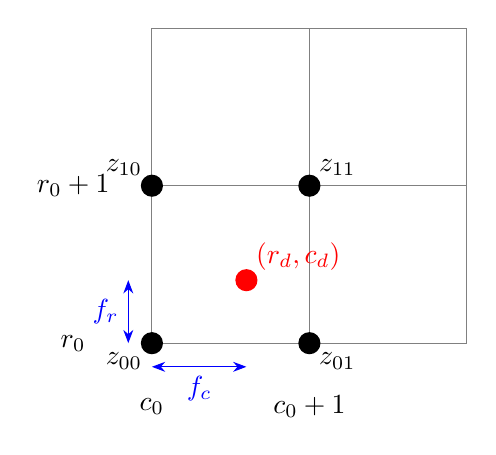
\begin{tikzpicture}[scale=2]
    % Grid
    \draw[gray,thin] (0,0) grid (2,2);

    % Corner points
    \fill (0,0) circle (2pt) node[below left] {$z_{00}$};
    \fill (1,0) circle (2pt) node[below right] {$z_{01}$};
    \fill (0,1) circle (2pt) node[above left] {$z_{10}$};
    \fill (1,1) circle (2pt) node[above right] {$z_{11}$};

    % Interpolation point
    \fill[red] (0.6,0.4) circle (2pt) node[above right] {$(r_d, c_d)$};

    % Fractional distances
    \draw[{Stealth}-{Stealth},blue] (0,-0.15) -- (0.6,-0.15) node[midway,below] {$f_c$};
    \draw[{Stealth}-{Stealth},blue] (-0.15,0) -- (-0.15,0.4) node[midway,left] {$f_r$};

    % Pixel coordinates
    \node at (0,-0.4) {$c_0$};
    \node at (1,-0.4) {$c_0+1$};
    \node at (-0.5,0) {$r_0$};
    \node at (-0.5,1) {$r_0+1$};
\end{tikzpicture}
\caption{Bilinear interpolation: The value at $(r_d, c_d)$ is computed as a weighted average of the four surrounding pixel values.}
\end{figure}

%=============================================================================
\section{Difference Image Calculation}
%=============================================================================

After registration, the difference image shows the per-pixel height difference between the aligned data and model:

\begin{equation}
\Delta z(r, c) = z_{\text{data}}^{\text{transformed}}(r, c) - z_{\text{model}}(r, c)
\end{equation}

For each valid model pixel $(r_m, c_m)$:
\begin{enumerate}
    \item Apply inverse transform to find corresponding data position
    \item Use bilinear interpolation to get data $z$-value
    \item Compute difference: $\Delta z = z_d + t_z - z_m$
\end{enumerate}

Pixels are marked as invalid if:
\begin{itemize}
    \item The transformed position falls outside the data image bounds
    \item Any of the four interpolation corners are invalid (holes)
    \item The pixel is outside the ROI
\end{itemize}

%=============================================================================
\section{Why Not Standard 3D ICP?}
%=============================================================================

Standard ICP fails for 2.5D data due to:

\subsection{Scale Imbalance}
With $z \approx 1000$ and $x, y \approx 0.01$, the $z$-axis dominates any 3D distance metric:
\begin{equation}
d_{3D} = \sqrt{(x_1-x_2)^2 + (y_1-y_2)^2 + (z_1-z_2)^2} \approx |z_1 - z_2|
\end{equation}

\subsection{Incorrect Correspondences}
3D nearest-neighbor finds points that are close in the $z$-direction, not points that correspond to the same physical location on the surface.

\begin{figure}[h]
\centering
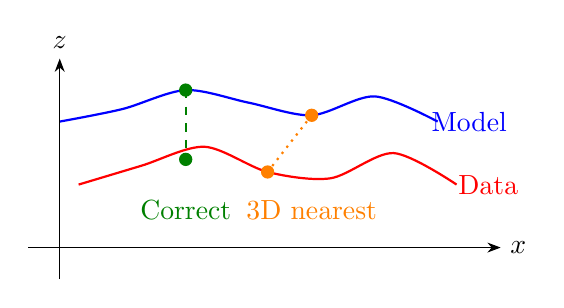
\begin{tikzpicture}[scale=0.8]
    % Model surface
    \draw[thick,blue] plot[smooth] coordinates {(0,2) (1,2.2) (2,2.5) (3,2.3) (4,2.1) (5,2.4) (6,2)};
    \node[blue] at (6.5,2) {Model};

    % Data surface (shifted)
    \draw[thick,red] plot[smooth] coordinates {(0.3,1) (1.3,1.3) (2.3,1.6) (3.3,1.2) (4.3,1.1) (5.3,1.5) (6.3,1)};
    \node[red] at (6.8,1) {Data};

    % Correct correspondence (vertical)
    \draw[green!50!black,thick,dashed] (2,2.5) -- (2,1.4);
    \fill[green!50!black] (2,2.5) circle (3pt);
    \fill[green!50!black] (2,1.4) circle (3pt);
    \node[green!50!black] at (2,0.6) {Correct};

    % Wrong correspondence (3D nearest)
    \draw[orange,thick,dotted] (4,2.1) -- (3.3,1.2);
    \fill[orange] (4,2.1) circle (3pt);
    \fill[orange] (3.3,1.2) circle (3pt);
    \node[orange] at (4,0.6) {3D nearest};

    % Axes
    \draw[-{Stealth}] (-0.5,0) -- (7,0) node[right] {$x$};
    \draw[-{Stealth}] (0,-0.5) -- (0,3) node[above] {$z$};
\end{tikzpicture}
\caption{Correspondence problem: 3D nearest-neighbor (orange) finds wrong correspondences. The correct correspondence (green) is based on $(x,y)$ position.}
\end{figure}

%=============================================================================
\section{References}
%=============================================================================

\begin{enumerate}
    \item Kanatani, K. (1994). ``Analysis of 3-D Rotation Fitting.'' \textit{IEEE Transactions on Pattern Analysis and Machine Intelligence}, 16(5), 543--549.

    \item Horn, B.K.P. (1987). ``Closed-form solution of absolute orientation using unit quaternions.'' \textit{Journal of the Optical Society of America A}, 4(4), 629--642.

    \item Besl, P.J. and McKay, N.D. (1992). ``A Method for Registration of 3-D Shapes.'' \textit{IEEE Transactions on Pattern Analysis and Machine Intelligence}, 14(2), 239--256.

    \item Eggert, D.W., Lorusso, A., and Fisher, R.B. (1997). ``Estimating 3-D rigid body transformations: a comparison of four major algorithms.'' \textit{Machine Vision and Applications}, 9(5-6), 272--290.
\end{enumerate}

\end{document}
